\newcommand{\TeamNo}{31}

\newcommand{\HWno}{03}

\newcommand{\AuthorOneName}{Merve Nur Öztürk}
\newcommand{\AuthorOneID}{2311322}

\newcommand{\AuthorTwoName}{Atakan Süslü}
\newcommand{\AuthorTwoID}{2311371}

\newcommand{\AuthorThreeName}{Betül Rana Kuran}
\newcommand{\AuthorThreeID}{2311173}


\documentclass[letterpaper,12pt]{article}
\usepackage{tabularx} % extra features for tabular environment
\usepackage{amsmath}  % improve math presentation
\usepackage{amssymb}
\usepackage{xcolor}
\usepackage{float}
\usepackage[export]{adjustbox}
\usepackage{graphicx} % takes care of graphic including machinery
\usepackage[margin=1in,letterpaper]{geometry} % decreases margins
\usepackage{cite} % takes care of citations

\begin{document}
\begin{center}
AE 305, 2020-21 Fall \hfill \textbf{HW \HWno} \hfill \textbf{Team \TeamNo} \\
\noindent\rule{\textwidth}{0.4pt}
\begin{tabular}{p{0.33\textwidth} | p{0.33\textwidth} | p{0.33\textwidth} }
	\AuthorOneName&\AuthorTwoName&\AuthorThreeName\\
	\textit{\AuthorOneID}&\textit{\AuthorTwoID}&\textit{\AuthorThreeID}
\end{tabular}
\noindent\rule{\textwidth}{0.4pt}
\end{center}

%Report start

\section{Introduction}
\label{section:intro}

Finite Volume Method is a numerical method used in order to solve partial differential
equations representing the conservation of a quantity. In this homework, potential flow
field over a circular cylinder at various values of angle of attack and a symmetric NACA
airfoil at zero angle of attack is requested to be calculated. For a potential flow,
velocity field is obtained by the Laplace's equation:

\begin{equation}
	\vec{\nabla} \cdot \vec{\nabla}\phi = \frac{\partial^2 \phi}{\partial x^2} + \frac{\partial^2 \phi}{\partial y^2} = 0.
\end{equation}

\begin{equation}
\vec{V} = \vec{\nabla}\phi
\end{equation}

A pseudo time derivative is introduced in order to solve this equation without a system
of linear algebraic equations.

\begin{equation}
	\frac{\partial \phi}{\partial t} = \nu \left(\frac{\partial^2 \phi}{\partial x^2} + \frac{\partial^2 \phi}{\partial y^2}\right)
\end{equation}

where $\nu$ is an artificial diffusion coefficient. Steady state boundary conditions are
set to calculate the steady state solution as the time derivative goes to zero during the
integration. The integral form of the above equation is:

\begin{equation}
	\frac{\partial}{\partial t} \int_{\Omega}\phi  d\Omega + \oint_{S} \vec{F} \cdot d\vec{S} = 0
\end{equation}

\begin{equation}
	\vec{F} = -\nu\frac{\partial \phi}{\partial x}\vec{i} - \nu\frac{\partial \phi}{\partial y}\vec{j}
\end{equation}

Two boundary conditions are set such that the velocity is equal to the free stream velocity
far away from the body (Farfield BC) and there is no flow normal to the body, which is no
penetration boundary condition (Wall BC):

\begin{eqnarray}
	\vec{\nabla}\phi|_{far BC} &=& \vec{V}_{\infty} = \vec{u}_{\infty}\vec{i} + \vec{v}_{\infty}\vec{j} = V_{\infty}(cos\alpha\vec{i}+sin\alpha\vec{j})\\
	&=& V_{\infty}cos\alpha\vec{i} + V_{\infty}sin\alpha\vec{j}
\end{eqnarray}

\begin{equation}
	(\vec{n}\cdot\vec{V}_{\infty})_{wall} = 0 or (\vec{F}\cdot\vec{S})_{wall} = 0.
\end{equation}

The conserved quantity for this problem is the potential $\phi$, and the FV method is applied
for the calculation of this quantity as explained above.



\section{Method}

\newpage

\section{Results and Discussion}
\subsection{Flowfield Around A Cylinder}

\begin{figure} [ht]
	\centering
	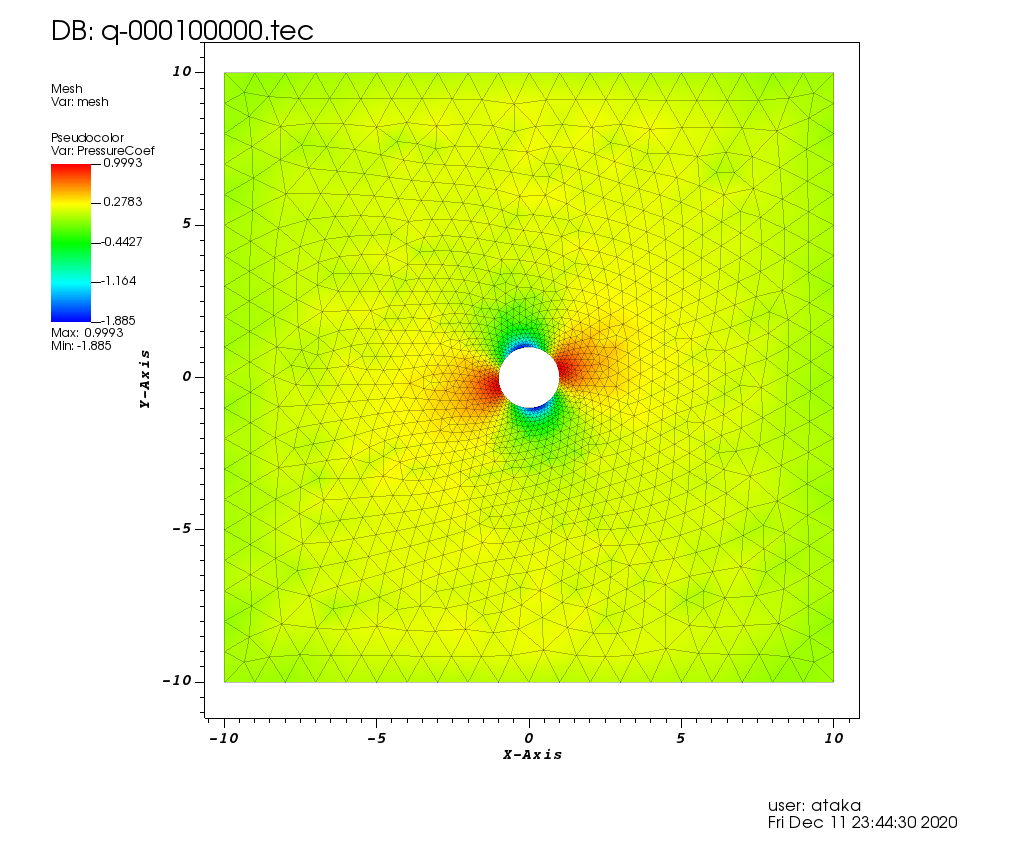
\includegraphics[height = 10cm]{graph/15deg/Cylinder_15angle_pressure0000.png}
	\caption{Potential flow over a circular cylinder at $\alpha=15$ calculated by FV method.}
    \label{fig:q1pc}
\end{figure}

According to the boundary conditions mentioned in Section \ref{section:adaptive}, FV fortran code
is completed. Afterwards, flowfield around a cylinder calculated using the unstructured grid provided.


\section{Conclusion}

\end{document}